\documentclass{report}
\usepackage[margin=2cm, bottom=1.5cm]{geometry}
\usepackage{type1cm}
\usepackage{amssymb}
\usepackage[fleqn]{amsmath}
\usepackage{tikz}
\usepackage{multicol}
\usepackage{makecell}
\usepackage{tabularx}
\usepackage[shortlabels]{enumitem}
\setlength{\columnsep}{1pt}
\setlist[enumerate]{nosep}

\makeatletter
\newenvironment{myalign*}{\ifvmode\else\hfil\null\linebreak\fi
  \hspace*{-\leftmargin}\minipage\textwidth
  \setlength{\abovedisplayskip}{0pt}%
  \setlength{\abovedisplayshortskip}{\abovedisplayskip}%
  \start@align\@ne\st@rredtrue\m@ne}%
{\endalign\endminipage\linebreak}

\usepackage{xeCJK}
\setCJKmainfont{標楷體}

\begin{document}
\title{%
  \fontsize{40}{60}\selectfont
  SCAF  \\ % 
  \vspace*{2cm}%
  \fontsize{24}{30}\selectfont
  測試文件
}

\author{
  \fontsize{18}{28}\selectfont
  \begin{tabularx}{\textwidth}{
    |p{\dimexpr.25\linewidth-2\tabcolsep-1.33333\arrayrulewidth}%
    |p{\dimexpr.75\linewidth-2\tabcolsep-1.33333\arrayrulewidth}|%
  }
    \hline
    \centering 專案名稱 & SCAF 開發輔助工具 \\
    \hline
    \centering 撰寫日期 & 2022 / 12 / 22 \\
    \hline
    \centering 發展者 & 簡蔚驊 \! 鄧暐宣 \! 余威霆 \! 林佳何 \! 唐劭賢 \\
    \hline
  \end{tabularx}
}
\date{}
\usetikzlibrary{automata, positioning, arrows}
\maketitle
\tikzset{every state, accepting/.style={double distance=2pt}}

\fontsize{12}{18}\selectfont
\section*{1. 接測試目的與接受準則(Objectives and Acceptance Criteria)}
\subsection*{1.1 系統範圍(System Scope)}
  \begin{itemize}
    \item 完成進度
  \end{itemize}

\subsection*{1.2 測試接受準則(Test Acceptance Criteria)}
本測試計劃需要滿足下面的測試接受準則:\\
測試程序需要依照本測試計劃所訂定的程序進行,所有測試結果需要能符合預期測試結果方能接受。
  \begin{itemize}
    \item 當測試案例未通過時,相關模組開發之負責人需要進行程式修改(修復bug或改動功能),以能讓此案例重新通過測試。
    \item 重新進行測試時,測試人員需確認其他可能受影響的案例仍可正確執行。
  \end{itemize}


\section*{2. 測試環境(Testing Environment)}
\subsection*{2.1硬體需求(Hardware Specification and Configuration)}
\begin{tabularx}{\textwidth}{
  |p{\dimexpr.1\linewidth-2\tabcolsep-1.33333\arrayrulewidth}%
  |p{\dimexpr.3\linewidth-2\tabcolsep-1.33333\arrayrulewidth}%
  |p{\dimexpr.1\linewidth-2\tabcolsep-1.33333\arrayrulewidth}%
  |p{\dimexpr.3\linewidth-2\tabcolsep-1.33333\arrayrulewidth}%
  |p{\dimexpr.2\linewidth-2\tabcolsep-1.33333\arrayrulewidth}|%
}
  \hline
  項次 &  名稱 & 數量 & 規格  & 備註  \\ \hline
  1 & TUF Gaming FX507ZM & 1 & 16G RAM, 512G SSD & window系統  \\ \hline
  2 & ROG Zephyrus GA503QS & 1 & 16G RAM, 512G SSD & window系統  \\ \hline
  3 & ThinkPad E15 Gen 4 & 1 & 8G RAM, 512G SSD & window系統  \\ \hline
  4 & ThinkPad E15 Gen 4 & 1 & 16G RAM, 512G SSD & window系統  \\ \hline
  
\end{tabularx}

\subsection*{2.2軟體需求(Hardware Specification and Configuration)}
\begin{tabularx}{\textwidth}{ 
  |p{\dimexpr.1\linewidth-2\tabcolsep-1.33333\arrayrulewidth}%
  |p{\dimexpr.3\linewidth-2\tabcolsep-1.33333\arrayrulewidth}%
  |p{\dimexpr.1\linewidth-2\tabcolsep-1.33333\arrayrulewidth}%
  |p{\dimexpr.3\linewidth-2\tabcolsep-1.33333\arrayrulewidth}%
  |p{\dimexpr.2\linewidth-2\tabcolsep-1.33333\arrayrulewidth}|%
}
  \hline
  項次 &  名稱 & 數量 & 規格  & 備註  \\
  \hline
  1 & chrome & 1 & 版本 108.0.5359.125 & clinet端瀏覽器  \\
  \hline
  2 & Firebase & 1 & 版本 11.4.0 & server端資料庫  \\
  \hline
\end{tabularx}

\section*{3. 測試案例(Test Cases)}
\begin{tabularx}{\textwidth}{
  |p{\dimexpr.25\linewidth-2\tabcolsep-1.33333\arrayrulewidth}%
  |p{\dimexpr.75\linewidth-2\tabcolsep-1.33333\arrayrulewidth}|%
  }
  \hline
  \centering Identification &  SCAF-TC-01 \\
  \hline
  \centering Name & 登入帳號測試 \\
  \hline
  \centering Reference & SCAF-FR-01 \\
  \hline
  \centering Severity & 高 \\
  \hline
  \centering Instructions & 
  \makecell[l]{
    1. 輸入網址進入SCAF系統 \\
    2. 輸入已註冊過的使用者信箱及密碼 \\
    3. 點擊 Sign in
  }\\
  \hline
  \centering Expected result & 成功登入系統,並能在setting頁面看到正確使用者資訊 \\
  \hline
  \centering Cleanup & 無 \\
  \hline
\end{tabularx}
\newline\newline
\begin{tabularx}{\textwidth}{
  |p{\dimexpr.25\linewidth-2\tabcolsep-1.33333\arrayrulewidth}%
  |p{\dimexpr.75\linewidth-2\tabcolsep-1.33333\arrayrulewidth}|%
  }
  \hline
  \centering Identification &  SCAF-TC-02 \\
  \hline
  \centering Name & 登入帳號測試 \\
  \hline
  \centering Reference & SCAF-FR-01 \\
  \hline
  \centering Severity & 高 \\
  \hline
  \centering Instructions & 
  \makecell[l]{
    1. 輸入網址進入SCAF系統 \\
    2. 輸入存在可未註冊的使用者信箱及密碼 EX: Gmail + 密碼 \\
    3. 點擊 Sign in
  }\\
  \hline
  \centering Expected result & 系統顯示錯誤的使用者名稱或密碼 \\
  \hline
  \centering Cleanup & 無 \\
  \hline
\end{tabularx}
\\
\newline
\\
\begin{tabularx}{\textwidth}{
  |p{\dimexpr.25\linewidth-2\tabcolsep-1.33333\arrayrulewidth}%
  |p{\dimexpr.75\linewidth-2\tabcolsep-1.33333\arrayrulewidth}|%
  }
  \hline
  \centering Identification &  SCAF-TC-03 \\
  \hline
  \centering Name & 註冊帳號測試 \\
  \hline
  \centering Reference & SCAF-FR-02 \\
  \hline
  \centering Severity & 高 \\
  \hline
  \centering Instructions & 
  \makecell[l]{
    1. 在登入頁面點選Sign Up進入註冊頁面 \\
    2. 輸入存在可未註冊的使用者信箱及密碼 EX: Gmail + 密碼 \\
    3. 點擊 Sign Up
    4. 輸入剛註冊完的信箱及密碼
    5. 點擊 Sign in
  }\\
  \hline
  \centering Expected result & 系統顯示註冊成功,並成功登入系統 \\
  \hline
  \centering Cleanup & 無 \\
  \hline
\end{tabularx}
\\
\newline
\\
\begin{tabularx}{\textwidth}{
  |p{\dimexpr.25\linewidth-2\tabcolsep-1.33333\arrayrulewidth}%
  |p{\dimexpr.75\linewidth-2\tabcolsep-1.33333\arrayrulewidth}|%
  }
  \hline
  \centering Identification &  SCAF-TC-04 \\
  \hline
  \centering Name & 註冊帳號測試 \\
  \hline
  \centering Reference & SCAF-FR-02 \\
  \hline
  \centering Severity & 中 \\
  \hline
  \centering Instructions & 
  \makecell[l]{
    1. 在登入頁面點選Sign Up進入註冊頁面 \\
    2. 輸入不符合格式的信箱或已被註冊過的信箱  \\
    3. 點擊 Sign Up
  }\\
  \hline
  \centering Expected result & 系統顯示註冊失敗,要求使用者重新輸入 \\
  \hline
  \centering Cleanup & 無 \\
  \hline
\end{tabularx}
\\
\newline
\\
\begin{tabularx}{\textwidth}{
  |p{\dimexpr.25\linewidth-2\tabcolsep-1.33333\arrayrulewidth}%
  |p{\dimexpr.75\linewidth-2\tabcolsep-1.33333\arrayrulewidth}|%
  }
  \hline
  \centering Identification &  SCAF-TC-05 \\
  \hline
  \centering Name & 忘記密碼測試 \\
  \hline
  \centering Reference & SCAF-FR-03 \\
  \hline
  \centering Severity & 高 \\
  \hline
  \centering Instructions & 
  \makecell[l]{
    1. 在登入頁面點選Forgot Password?進入重設密碼頁面 \\
    2. 輸入已註冊過的信箱  \\
    3. 點擊Submit \\
    4. 在信箱中確認Firebase發送的重設密碼信件 \\
    5. 輸入新的密碼 \\
    6. 回到登入頁面輸入更改後的密碼  \\
    7. 點擊 Sign in
  }\\
  \hline
  \centering Expected result & 在信箱中成功接收Firebase的信件,並在修改過後成功登入系統 \\
  \hline
  \centering Cleanup & 無 \\
  \hline
\end{tabularx}
\\
\newline
\\
\begin{tabularx}{\textwidth}{
  |p{\dimexpr.25\linewidth-2\tabcolsep-1.33333\arrayrulewidth}%
  |p{\dimexpr.75\linewidth-2\tabcolsep-1.33333\arrayrulewidth}|%
  }
  \hline
  \centering Identification &  SCAF-TC-06 \\
  \hline
  \centering Name & 忘記密碼測試 \\
  \hline
  \centering Reference & SCAF-FR-03 \\
  \hline
  \centering Severity & 中 \\
  \hline
  \centering Instructions & 
  \makecell[l]{
    1. 在登入頁面點選Forgot Password?進入重設密碼頁面 \\
    2. 輸入未註冊過的信箱  \\
    3. 點擊Submit
    4. 在信箱中確認Firebase發送的重設密碼信件
  }\\
  \hline
  \centering Expected result & 確認信箱中未出現信件 \\
  \hline
  \centering Cleanup & 無 \\
  \hline
\end{tabularx}
\\
\newline
\\
\begin{tabularx}{\textwidth}{
  |p{\dimexpr.25\linewidth-2\tabcolsep-1.33333\arrayrulewidth}%
  |p{\dimexpr.75\linewidth-2\tabcolsep-1.33333\arrayrulewidth}|%
  }
  \hline
  \centering Identification &  SCAF-TC-07 \\
  \hline
  \centering Name & 共用專案測試 \\
  \hline
  \centering Reference & SCAF-FR-04 \\
  \hline
  \centering Severity & 中 \\
  \hline
  \centering Instructions & 
  \makecell[l]{
    1. 專案擁有者點擊My project到專案列表頁面 \\
    2. 點選隨意一個專案進入到專案中 \\
    3. 專案擁有者點擊Project名稱下方的Setting \\
    4. 輸入已註冊過的使用者信箱 \\
    5. 接收者點擊通知中的專案邀請訊息 \\
    6. 接收者點擊確認加入專案 \\
    7. 接收者點擊navrbar的My project回到專案列表 \\
    8. 進入專案查看其他專案資訊
  }\\
  \hline
  \centering Expected result & 接收者的專案列表中,成功出現接收邀請的專案,且專案內容皆與擁有者相同 \\
  \hline
  \centering Cleanup & 無 \\
  \hline
\end{tabularx}
\\
\newline
\\
\begin{tabularx}{\textwidth}{
  |p{\dimexpr.25\linewidth-2\tabcolsep-1.33333\arrayrulewidth}%
  |p{\dimexpr.75\linewidth-2\tabcolsep-1.33333\arrayrulewidth}|%
  }
  \hline
  \centering Identification &  SCAF-TC-08 \\
  \hline
  \centering Name & 更改專案內容測試 \\
  \hline
  \centering Reference & SCAF-FR-04 \\
  \hline
  \centering Severity & 高 \\
  \hline
  \centering Instructions & 
  \makecell[l]{
    1. 點擊My project到專案列表頁面 \\
    2. 點選隨意一個專案進入到專案中 \\
    3. 點擊專案名稱下方的documnet \\
    4. 按下edit \\
    5. 在codimd中編輯檔案
  }\\
  \hline
  \centering Expected result & 其餘專案成員皆能看見檔案的變更 \\
  \hline
  \centering Cleanup & 無 \\
  \hline
\end{tabularx}
\\
\newline
\\
\begin{tabularx}{\textwidth}{
  |p{\dimexpr.25\linewidth-2\tabcolsep-1.33333\arrayrulewidth}%
  |p{\dimexpr.75\linewidth-2\tabcolsep-1.33333\arrayrulewidth}|%
  }
  \hline
  \centering Identification &  SCAF-TC-09 \\
  \hline
  \centering Name & 刪除專案測試 \\
  \hline
  \centering Reference & SCAF-FR-04 \\
  \hline
  \centering Severity & 高 \\
  \hline
  \centering Instructions & 
  \makecell[l]{
    1. 專案擁有者點擊My project到專案列表頁面 \\
    2. 專案擁有者點擊專案的X進行刪除專案 \\
    3. 專案內的成員查看專案列表頁面 
  }\\
  \hline
  \centering Expected result & 專案內的所有成員此專案皆被刪除(未再顯示在專案列表上) \\
  \hline
  \centering Cleanup & 無 \\
  \hline
\end{tabularx}
\\
\newline
\\
\begin{tabularx}{\textwidth}{
  |p{\dimexpr.25\linewidth-2\tabcolsep-1.33333\arrayrulewidth}%
  |p{\dimexpr.75\linewidth-2\tabcolsep-1.33333\arrayrulewidth}|%
  }
  \hline
  \centering Identification &  SCAF-TC-10 \\
  \hline
  \centering Name & 刪除專案測試 \\
  \hline
  \centering Reference & SCAF-FR-04 \\
  \hline
  \centering Severity & 中 \\
  \hline
  \centering Instructions & 
  \makecell[l]{
    1. 專案成員點擊My project到專案列表頁面 \\
    2. 專案成員點擊專案的X進行刪除專案 \\
    3. 專案內的成員查看專案列表頁面  
  }\\
  \hline
  \centering Expected result & 系統顯示使用者並非專案擁有者不可刪除專案,且專案成員的專案列表上此專案並未被刪除 \\
  \hline
  \centering Cleanup & 無 \\
  \hline
\end{tabularx}
\\
\newline
\\
\begin{tabularx}{\textwidth}{
  |p{\dimexpr.25\linewidth-2\tabcolsep-1.33333\arrayrulewidth}%
  |p{\dimexpr.75\linewidth-2\tabcolsep-1.33333\arrayrulewidth}|%
  }
  \hline
  \centering Identification &  SCAF-TC-11 \\
  \hline
  \centering Name & 開發流程測試 \\
  \hline
  \centering Reference & SCAF-FR-05 \\
  \hline
  \centering Severity & 低 \\
  \hline
  \centering Instructions & 
  \makecell[l]{
    1. 專案擁有者點擊Project名稱下方的Setting \\
    2. 專案成員選擇瀑布式開發或敏捷式開發 \\
  }\\
  \hline
  \centering Expected result & 系統跳出兩個流程的的執行方法,並舉例設定流程日期的方式 \\
  \hline
  \centering Cleanup & 無 \\
  \hline
\end{tabularx}
\\
\newline
\\
\begin{tabularx}{\textwidth}{
  |p{\dimexpr.25\linewidth-2\tabcolsep-1.33333\arrayrulewidth}%
  |p{\dimexpr.75\linewidth-2\tabcolsep-1.33333\arrayrulewidth}|%
  }
  \hline
  \centering Identification &  SCAF-TC-12 \\
  \hline
  \centering Name & 專案初始化測試 \\
  \hline
  \centering Reference & SCAF-FR-06 \\
  \hline
  \centering Severity & 中 \\
  \hline
  \centering Instructions & 
  \makecell[l]{
    1. 點擊My project到專案列表頁面  \\
    2. 點擊+號創建一個新的專案  \\
    3. 輸入名稱、選擇加入README檔  \\
    4. 按下Create
  }\\
  \hline
  \centering Expected result & 專案內document有README檔、專案列表有新增該檔案 \\
  \hline
  \centering Cleanup & 無 \\
  \hline
\end{tabularx}
\\
\newline
\\
\begin{tabularx}{\textwidth}{
  |p{\dimexpr.25\linewidth-2\tabcolsep-1.33333\arrayrulewidth}%
  |p{\dimexpr.75\linewidth-2\tabcolsep-1.33333\arrayrulewidth}|%
  }
  \hline
  \centering Identification &  SCAF-TC-13 \\
  \hline
  \centering Name & 專案初始化測試 \\
  \hline
  \centering Reference & SCAF-FR-06 \\
  \hline
  \centering Severity & 中 \\
  \hline
  \centering Instructions & 
  \makecell[l]{
    1. 點擊My project到專案列表頁面  \\
    2. 點擊+號創建一個新的專案  \\
    3. 輸入名稱、不選擇加入README檔  \\
    4. 按下Create
  }\\
  \hline
  \centering Expected result & 專案內document沒有README檔、專案列表有新增該檔案 \\
  \hline
  \centering Cleanup & 無 \\
  \hline
\end{tabularx}
\\
\newline
\\
\begin{tabularx}{\textwidth}{
  |p{\dimexpr.25\linewidth-2\tabcolsep-1.33333\arrayrulewidth}%
  |p{\dimexpr.75\linewidth-2\tabcolsep-1.33333\arrayrulewidth}|%
  }
  \hline
  \centering Identification &  SCAF-TC-14 \\
  \hline
  \centering Name & 新增repository \\
  \hline
  \centering Reference & SCAF-FR-07 \\
  \hline
  \centering Severity & 高 \\
  \hline
  \centering Instructions & 
  \makecell[l]{
    1. 點擊專案列表隨意一個專案 \\
    2. 點擊專案名稱下方的repositories \\
    3. 點擊+號創建一個新的repository \\
    3. 輸入repository 名稱、對應的github網址  \\
    4. 按下Create
  }\\
  \hline
  \centering Expected result & repository列表應新增此repository,點擊連結能夠跳轉到對應的網址 \\
  \hline
  \centering Cleanup & 無 \\
  \hline
\end{tabularx}
\\
\newline
\\
\begin{tabularx}{\textwidth}{
  |p{\dimexpr.25\linewidth-2\tabcolsep-1.33333\arrayrulewidth}%
  |p{\dimexpr.75\linewidth-2\tabcolsep-1.33333\arrayrulewidth}|%
  }
  \hline
  \centering Identification &  SCAF-TC-15 \\
  \hline
  \centering Name & 新增repository \\
  \hline
  \centering Reference & SCAF-FR-07 \\
  \hline
  \centering Severity & 低 \\
  \hline
  \centering Instructions & 
  \makecell[l]{
    1. 點擊專案列表隨意一個專案 \\
    2. 點擊專案名稱下方的repositories \\
    3. 點擊+號創建一個新的repository \\
    3. 輸入repository 名稱、不存在的github網址  \\
    4. 按下Create
  }\\
  \hline
  \centering Expected result & 系統顯示此連結網址無效,請重新輸入 \\
  \hline
  \centering Cleanup & 無 \\
  \hline
\end{tabularx}
\\
\newline
\\
\begin{tabularx}{\textwidth}{
  |p{\dimexpr.25\linewidth-2\tabcolsep-1.33333\arrayrulewidth}%
  |p{\dimexpr.75\linewidth-2\tabcolsep-1.33333\arrayrulewidth}|%
  }
  \hline
  \centering Identification &  SCAF-TC-16 \\
  \hline
  \centering Name & 刪除repository \\
  \hline
  \centering Reference & SCAF-FR-07 \\
  \hline
  \centering Severity & 高 \\
  \hline
  \centering Instructions & 
  \makecell[l]{
    1. 點擊專案名稱下方的repositories \\
    2. 點擊repository旁邊的X刪除repository \\
  }\\
  \hline
  \centering Expected result & 此repository在repositories列表中消失 \\
  \hline
  \centering Cleanup & 無 \\
  \hline
\end{tabularx}
\\
\newline
\\
\begin{tabularx}{\textwidth}{
  |p{\dimexpr.25\linewidth-2\tabcolsep-1.33333\arrayrulewidth}%
  |p{\dimexpr.75\linewidth-2\tabcolsep-1.33333\arrayrulewidth}|%
  }
  \hline
  \centering Identification &  SCAF-TC-17 \\
  \hline
  \centering Name & 預覽文件測試 \\
  \hline
  \centering Reference & SCAF-FR-08 \\
  \hline
  \centering Severity & 中 \\
  \hline
 \centering Instructions & 
  \makecell[l]{
    1. 點擊專案名稱下方的documnet \\
    2. 在畫面中瀏覽已存在的檔案
  }\\
  \hline
  \centering Expected result & 檔案呈現唯獨狀態,顯示在頁面上 \\
  \hline
  \centering Cleanup & 無 \\
  \hline
\end{tabularx}
\\
\newline
\\
\begin{tabularx}{\textwidth}{
  |p{\dimexpr.25\linewidth-2\tabcolsep-1.33333\arrayrulewidth}%
  |p{\dimexpr.75\linewidth-2\tabcolsep-1.33333\arrayrulewidth}|%
  }
  \hline
  \centering Identification &  SCAF-TC-18 \\
  \hline
  \centering Name & 預覽文件測試 \\
  \hline
  \centering Reference & SCAF-FR-08 \\
  \hline
  \centering Severity & 中 \\
  \hline
 \centering Instructions & 
  \makecell[l]{
    1. 點擊專案名稱下方的documnet \\
    2. 在畫面中瀏覽尚未建立的檔案
  }\\
  \hline
  \centering Expected result & 預覽區塊為空,提示專案人員尚未建立檔案 \\
  \hline
  \centering Cleanup & 無 \\
  \hline
\end{tabularx}
\\
\newline
\\
\begin{tabularx}{\textwidth}{
  |p{\dimexpr.25\linewidth-2\tabcolsep-1.33333\arrayrulewidth}%
  |p{\dimexpr.75\linewidth-2\tabcolsep-1.33333\arrayrulewidth}|%
  }
  \hline
  \centering Identification &  SCAF-TC-19 \\
  \hline
  \centering Name & 編輯文件測試 \\
  \hline
  \centering Reference & SCAF-FR-08 \\
  \hline
  \centering Severity & 高 \\
  \hline
  \centering Instructions & 
  \makecell[l]{
    1. 點擊documnet頁面中需求文件的edit(若不存在會直接建立) \\
    2. 更改該文件內容  \\
    3. 存檔  \\
    4. 返回document頁面
  }\\
  \hline
  \centering Expected result & 預覽頁面應顯示更動內容 \\
  \hline
  \centering Cleanup & 無 \\
  \hline
\end{tabularx}
\\
\newline
\\
\begin{tabularx}{\textwidth}{
  |p{\dimexpr.25\linewidth-2\tabcolsep-1.33333\arrayrulewidth}%
  |p{\dimexpr.75\linewidth-2\tabcolsep-1.33333\arrayrulewidth}|%
  }
  \hline
  \centering Identification &  SCAF-TC-20 \\
  \hline
  \centering Name & 編輯文件測試 \\
  \hline
  \centering Reference & SCAF-FR-08 \\
  \hline
  \centering Severity & 低 \\
  \hline
  \centering Instructions & 
  \makecell[l]{
    1. 點擊documnet頁面中需求文件的edit(若不存在會直接建立) \\
    2. 更改該文件內容  \\
    3. 不存檔直接退出  \\
    4. 返回document頁面
  }\\
  \hline
  \centering Expected result & 預覽頁面應顯示未修改的畫面 \\
  \hline
  \centering Cleanup & 無 \\
  \hline
\end{tabularx}
\\
\newline
\\
\begin{tabularx}{\textwidth}{
  |p{\dimexpr.25\linewidth-2\tabcolsep-1.33333\arrayrulewidth}%
  |p{\dimexpr.75\linewidth-2\tabcolsep-1.33333\arrayrulewidth}|%
  }
  \hline
  \centering Identification &  SCAF-TC-21 \\
  \hline
  \centering Name & 新增一個任務至看板中 \\
  \hline
  \centering Reference & SCAF-FR-09 \\
  \hline
  \centering Severity & 高 \\
  \hline
  \centering Instructions & 
  \makecell[l]{
    1. 點擊專案名稱下方的Kanban  \\
    2. 按下 TO DO 旁邊的+  \\
    3. 填入任務名稱、選擇分配人員  \\
    4. 按下Create
  }\\
  \hline
  \centering Expected result & TO DO下方應增加一個任務,包含名稱和其分配人員 \\
  \hline
  \centering Cleanup & 無 \\
  \hline
\end{tabularx}
\\
\newline
\\
\begin{tabularx}{\textwidth}{
  |p{\dimexpr.25\linewidth-2\tabcolsep-1.33333\arrayrulewidth}%
  |p{\dimexpr.75\linewidth-2\tabcolsep-1.33333\arrayrulewidth}|%
  }
  \hline
  \centering Identification &  SCAF-TC-22 \\
  \hline
  \centering Name & 新增一個任務至看板中 \\
  \hline
  \centering Reference & SCAF-FR-09 \\
  \hline
  \centering Severity & 低 \\
  \hline
  \centering Instructions & 
  \makecell[l]{
    1. 點擊專案名稱下方的Kanban  \\
    2. 按下 TO DO 旁邊的+  \\
    3. 填入任務名稱、未選擇分配人員  \\
    4. 按下Create
  }\\
  \hline
  \centering Expected result & 系統應提示請分派人員負責此工作,且不會出現在看板中 \\
  \hline
  \centering Cleanup & 無 \\
  \hline
\end{tabularx}
\\
\newline
\\
\begin{tabularx}{\textwidth}{
  |p{\dimexpr.25\linewidth-2\tabcolsep-1.33333\arrayrulewidth}%
  |p{\dimexpr.75\linewidth-2\tabcolsep-1.33333\arrayrulewidth}|%
  }
  \hline
  \centering Identification &  SCAF-TC-23 \\
  \hline
  \centering Name & 移動看板中的任務 \\
  \hline
  \centering Reference & SCAF-FR-09 \\
  \hline
  \centering Severity & 高 \\
  \hline
  \centering Instructions & 
  \makecell[l]{
    1. 拖曳Doing下方任一個任務  \\
    2. 在Done的位置放開滑鼠 
  }\\
  \hline
  \centering Expected result & 此任務消失在Doing欄位,並出現在Done \\
  \hline
  \centering Cleanup & 無 \\
  \hline
\end{tabularx}
\\
\newline
\\
\begin{tabularx}{\textwidth}{
  |p{\dimexpr.25\linewidth-2\tabcolsep-1.33333\arrayrulewidth}%
  |p{\dimexpr.75\linewidth-2\tabcolsep-1.33333\arrayrulewidth}|%
  }
  \hline
  \centering Identification &  SCAF-TC-24 \\
  \hline
  \centering Name & 移動看板中的任務 \\
  \hline
  \centering Reference & SCAF-FR-09 \\
  \hline
  \centering Severity & 低 \\
  \hline
  \centering Instructions & 
  \makecell[l]{
    1. 拖曳Doing下方任一個任務  \\
    2. 在Doing的位置放開滑鼠  \\
  }\\
  \hline
  \centering Expected result & 此頁面應無任何改變 \\
  \hline
  \centering Cleanup & 無 \\
  \hline
\end{tabularx}
\\
\newline
\\
\begin{tabularx}{\textwidth}{
  |p{\dimexpr.25\linewidth-2\tabcolsep-1.33333\arrayrulewidth}%
  |p{\dimexpr.75\linewidth-2\tabcolsep-1.33333\arrayrulewidth}|%
  }
  \hline
  \centering Identification &  SCAF-TC-25 \\
  \hline
  \centering Name & 接收通知 \\
  \hline
  \centering Reference & SCAF-FR-10 \\
  \hline
  \centering Severity & 低 \\
  \hline
  \centering Instructions & 
  \makecell[l]{
    1. 點擊documnet頁面中需求文件的edit \\
    2. 更改該文件內容  \\
    3. 存檔  \\
    4. 點擊Navrbar中的鈴鐺
  }\\
  \hline
  \centering Expected result & 需求文件更動的通知應顯示 \\
  \hline
  \centering Cleanup & 無 \\
  \hline
\end{tabularx}
\\
\newline
\\
\begin{tabularx}{\textwidth}{
  |p{\dimexpr.25\linewidth-2\tabcolsep-1.33333\arrayrulewidth}%
  |p{\dimexpr.75\linewidth-2\tabcolsep-1.33333\arrayrulewidth}|%
  }
  \hline
  \centering Identification &  SCAF-TC-26 \\
  \hline
  \centering Name & 專案邀請 \\
  \hline
  \centering Reference & SCAF-FR-10 \\
  \hline
  \centering Severity & 中 \\
  \hline
  \centering Instructions & 
  \makecell[l]{
    1. 專案擁有者點擊My project到專案列表頁面 \\
    2. 點選隨意一個專案進入到專案中 \\
    3. 專案擁有者點擊Project名稱下方的Setting \\
    4. 輸入已註冊過的使用者信箱 \\
    5. 接收者點擊Navrbar中的鈴鐺 \\
    6. 點擊專案邀請的訊息 
  }\\
  \hline
  \centering Expected result & 顯示專案名稱、邀請人、是否加入的選項 \\
  \hline
  \centering Cleanup & 無 \\
  \hline
\end{tabularx}
\\
\newline
\\
\begin{tabularx}{\textwidth}{
  |p{\dimexpr.25\linewidth-2\tabcolsep-1.33333\arrayrulewidth}%
  |p{\dimexpr.75\linewidth-2\tabcolsep-1.33333\arrayrulewidth}|%
  }
  \hline
  \centering Identification &  SCAF-TC-27 \\
  \hline
  \centering Name & 變更名稱、自介 \\
  \hline
  \centering Reference & SCAF-FR-11 \\
  \hline
  \centering Severity & 低 \\
  \hline
  \centering Instructions & 
  \makecell[l]{
    1. 點擊Navrbar中的Setting \\
    2. 填入新的名稱、自介 \\
    3. 點擊Save \\
    3. 重新點擊Setting頁面
  }\\
  \hline
  \centering Expected result & 顯示修改後的資料 \\
  \hline
  \centering Cleanup & 無 \\
  \hline
\end{tabularx}
\\
\newline
\\
\begin{tabularx}{\textwidth}{
  |p{\dimexpr.25\linewidth-2\tabcolsep-1.33333\arrayrulewidth}%
  |p{\dimexpr.75\linewidth-2\tabcolsep-1.33333\arrayrulewidth}|%
  }
  \hline
  \centering Identification &  SCAF-TC-28 \\
  \hline
  \centering Name & 變更密碼 \\
  \hline
  \centering Reference & SCAF-FR-11 \\
  \hline
  \centering Severity & 中 \\
  \hline
  \centering Instructions & 
  \makecell[l]{
    1. 點擊Navrbar中的Setting \\
    2. 點擊變更密碼 \\
    3. 在信箱中確認Firebase發送的重設密碼信件 \\
    4. 輸入新的密碼 \\
    5. 在終端機中輸入scaf signin\\
    6. 輸入信箱 \\
    7. 輸入新的密碼 \\
  }\\
  \hline
  \centering Expected result & 成功登入系統 \\
  \hline
  \centering Cleanup & 無 \\
  \hline
\end{tabularx}
\\
\newline
\\
\begin{tabularx}{\textwidth}{
  |p{\dimexpr.25\linewidth-2\tabcolsep-1.33333\arrayrulewidth}%
  |p{\dimexpr.75\linewidth-2\tabcolsep-1.33333\arrayrulewidth}|%
  }
  \hline
  \centering Identification &  SCAF-TC-29 \\
  \hline
  \centering Name & 變更密碼 \\
  \hline
  \centering Reference & SCAF-FR-11 \\
  \hline
  \centering Severity & 中 \\
  \hline
  \centering Instructions & 
  \makecell[l]{
    1. 點擊Navrbar中的Setting \\
    2. 填入新的密碼 \\
    3. 點擊Save \\
    4. 登出 \\
    5. 輸入信箱、原始的密碼
  }\\
  \hline
  \centering Expected result & 系統顯示密碼錯誤 \\
  \hline
  \centering Cleanup & 無 \\
  \hline
\end{tabularx}
\\
\newline
\\
\begin{tabularx}{\textwidth}{
  |p{\dimexpr.25\linewidth-2\tabcolsep-1.33333\arrayrulewidth}%
  |p{\dimexpr.75\linewidth-2\tabcolsep-1.33333\arrayrulewidth}|%
  }
  \hline
  \centering Identification &  SCAF-TC-30 \\
  \hline
  \centering Name & 查看Q\&A \\
  \hline
  \centering Reference & SCAF-FR-12 \\
  \hline
  \centering Severity & 高 \\
  \hline
  \centering Instructions & 
  \makecell[l]{
    1. 點擊Navrbar中的Q\&A
  }\\
  \hline
  \centering Expected result & 顯示GitBook的內容 \\
  \hline
  \centering Cleanup & 無 \\
  \hline
\end{tabularx}
\\
\newline
\\
% \begin{tabularx}{\textwidth}{
%   |p{\dimexpr.25\linewidth-2\tabcolsep-1.33333\arrayrulewidth}%
%   |p{\dimexpr.75\linewidth-2\tabcolsep-1.33333\arrayrulewidth}|%
%   }
%   \hline
%   \centering Identification &  SCAF-TC-28 \\
%   \hline
%   \centering Name & Google 日曆授權 \\
%   \hline
%   \centering Reference & SCAF-FR-13 \\
%   \hline
%   \centering Severity & 1 \\
%   \hline
%   \centering Instructions & 
%   \makecell[l]{
%     1. 點擊Navrbar中的Setting \\
%     2. 點擊Google日曆旁的授權按鈕 \\
%     3. 按下授權 
%   }\\
%   \hline
%   \centering Expected result & 成功連結Google日曆 \\
%   \hline
%   \centering Cleanup & 無 \\
%   \hline
% \end{tabularx}
%\\
%\newline
%\\
% \begin{tabularx}{\textwidth}{
%   |p{\dimexpr.25\linewidth-2\tabcolsep-1.33333\arrayrulewidth}%
%   |p{\dimexpr.75\linewidth-2\tabcolsep-1.33333\arrayrulewidth}|%
%   }
%   \hline
%   \centering Identification &  SCAF-TC-29 \\
%   \hline
%   \centering Name & Google 日曆授權 \\
%   \hline
%   \centering Reference & SCAF-FR-13 \\
%   \hline
%   \centering Severity & 1 \\
%   \hline
%   \centering Instructions & 
%   \makecell[l]{
%     1. 點擊Navrbar中的Setting \\
%     2. 點擊Google日曆旁的授權按鈕 \\
%     3. 按下取消 
%   }\\
%   \hline
%   \centering Expected result & 未連結Google日曆 \\
%   \hline
%   \centering Cleanup & 無 \\
%   \hline
% \end{tabularx}
%\\
%\newline
%\\
\begin{tabularx}{\textwidth}{
  |p{\dimexpr.25\linewidth-2\tabcolsep-1.33333\arrayrulewidth}%
  |p{\dimexpr.75\linewidth-2\tabcolsep-1.33333\arrayrulewidth}|%
  }
  \hline
  \centering Identification &  SCAF-TC-31 \\
  \hline
  \centering Name & 變更專案名稱 \\
  \hline
  \centering Reference & SCAF-FR-14 \\
  \hline
  \centering Severity & 低 \\
  \hline
  \centering Instructions & 
  \makecell[l]{
    1. 點擊專案名稱下方的setting \\
    2. 點擊general頁面 \\
    3. 輸入新的專案名稱 \\
    4. 按下Update 
  }\\
  \hline
  \centering Expected result & 頁面、專案列表名稱皆更動成新的名稱 \\
  \hline
  \centering Cleanup & 無 \\
  \hline
\end{tabularx}
\\
\newline
\\
\begin{tabularx}{\textwidth}{
  |p{\dimexpr.25\linewidth-2\tabcolsep-1.33333\arrayrulewidth}%
  |p{\dimexpr.75\linewidth-2\tabcolsep-1.33333\arrayrulewidth}|%
  }
  \hline
  \centering Identification &  SCAF-TC-32 \\
  \hline
  \centering Name & 新增專案成員 \\
  \hline
  \centering Reference & SCAF-FR-14 \\
  \hline
  \centering Severity & 中 \\
  \hline
  \centering Instructions & 
  \makecell[l]{
    1. 專案擁有者點擊Project名稱下方的Setting \\
    2. 輸入已註冊過的使用者信箱 \\
    3. 接收者點擊通知中的專案邀請訊息 \\
    4. 接收者點擊確認加入專案 \\
    5. 專案擁有者確認member頁面
  }\\
  \hline
  \centering Expected result & 應增加加入者之訊息 \\
  \hline
  \centering Cleanup & 無 \\
  \hline
\end{tabularx}
\\
\newline
\\
\begin{tabularx}{\textwidth}{
  |p{\dimexpr.25\linewidth-2\tabcolsep-1.33333\arrayrulewidth}%
  |p{\dimexpr.75\linewidth-2\tabcolsep-1.33333\arrayrulewidth}|%
  }
  \hline
  \centering Identification &  SCAF-TC-33 \\
  \hline
  \centering Name & 剔除專案成員 \\
  \hline
  \centering Reference & SCAF-FR-14 \\
  \hline
  \centering Severity & 低 \\
  \hline
  \centering Instructions & 
  \makecell[l]{
    1. 專案擁有者點擊Project名稱下方的Setting \\
    2. 點擊任一位專案成員旁的X
    3. 被剔除人員確認專案列表
  }\\
  \hline
  \centering Expected result & 此專案應消失在專案列表中 \\
  \hline
  \centering Cleanup & 無 \\
  \hline
\end{tabularx}
\\
\newline
\\
\begin{tabularx}{\textwidth}{
  |p{\dimexpr.25\linewidth-2\tabcolsep-1.33333\arrayrulewidth}%
  |p{\dimexpr.75\linewidth-2\tabcolsep-1.33333\arrayrulewidth}|%
  }
  \hline
  \centering Identification &  SCAF-TC-34 \\
  \hline
  \centering Name & 專案初始化測試 \\
  \hline
  \centering Reference & SCAF-FR-06 \\
  \hline
  \centering Severity & 低 \\
  \hline
  \centering Instructions & 
  \makecell[l]{
    1. 點擊 My project 到專案列表頁面 \\
    2. 點擊 + 號創建一個新的專案 \\
    3. 輸入重複的專案名稱 \\
    4. 按下 Create
  }\\
  \hline
  \centering Expected result & 系統提示專案名稱已存在,專案列表未新增專案 \\
  \hline
  \centering Cleanup & 無 \\
  \hline
\end{tabularx}
\\
\newline
\\
\begin{tabularx}{\textwidth}{
  |p{\dimexpr.25\linewidth-2\tabcolsep-1.33333\arrayrulewidth}%
  |p{\dimexpr.75\linewidth-2\tabcolsep-1.33333\arrayrulewidth}|%
  }
  \hline
  \centering Identification &  SCAF-TC-35 \\
  \hline
  \centering Name & 專案初始化測試 \\
  \hline
  \centering Reference & SCAF-FR-06 \\
  \hline
  \centering Severity & 低 \\
  \hline
  \centering Instructions & 
  \makecell[l]{
    1. 點擊 My project 到專案列表頁面 \\
    2. 點擊 + 號創建一個新的專案 \\
    3. 輸入含非法字元的專案名稱 
    (如:/ \textbackslash ? \% * : |  " < >) \\
    4. 按下 Create
  }\\
  \hline
  \centering Expected result & 系統提示專案名稱不能有特殊字元,專案列表未新增專案 \\
  \hline
  \centering Cleanup & 無 \\
  \hline
\end{tabularx}
\\
\newline
\\
\begin{tabularx}{\textwidth}{
  |p{\dimexpr.25\linewidth-2\tabcolsep-1.33333\arrayrulewidth}%
  |p{\dimexpr.75\linewidth-2\tabcolsep-1.33333\arrayrulewidth}|%
  }
  \hline
  \centering Identification &  SCAF-TC-36\\
  \hline
  \centering Name & 登入帳號測試 \\
  \hline
  \centering Reference & SCAF-FR-01 \\
  \hline
  \centering Severity & 低 \\
  \hline
  \centering Instructions & 
  \makecell[l]{
    1. 輸入網址進入SCAF系統 \\
    2. 不輸入使用者信箱及密碼 \\
    3. 點擊 Sign in
  }\\
  \hline
  \centering Expected result & 系統顯示登入錯誤 \\
  \hline
  \centering Cleanup & 無 \\
  \hline
\end{tabularx}
\\
\newline
\\
\begin{tabularx}{\textwidth}{
  |p{\dimexpr.25\linewidth-2\tabcolsep-1.33333\arrayrulewidth}%
  |p{\dimexpr.75\linewidth-2\tabcolsep-1.33333\arrayrulewidth}|%
  }
  \hline
  \centering Identification &  SCAF-TC-37 \\
  \hline
  \centering Name & 註冊帳號測試 \\
  \hline
  \centering Reference & SCAF-FR-02 \\
  \hline
  \centering Severity & 低 \\
  \hline
  \centering Instructions & 
  \makecell[l]{
    1. 在登入頁面點選Sign Up進入註冊頁面 \\
    2. 不輸入使用者信箱及密碼  \\
    3. 點擊 Sign Up
  }\\
  \hline
  \centering Expected result & 系統顯示註冊錯誤 \\
  \hline
  \centering Cleanup & 無 \\
  \hline
\end{tabularx}
\\
\newline
\\
\begin{tabularx}{\textwidth}{
  |p{\dimexpr.25\linewidth-2\tabcolsep-1.33333\arrayrulewidth}%
  |p{\dimexpr.75\linewidth-2\tabcolsep-1.33333\arrayrulewidth}|%
  }
  \hline
  \centering Identification &  SCAF-TC-38 \\
  \hline
  \centering Name & 忘記密碼測試 \\
  \hline
  \centering Reference & SCAF-FR-03 \\
  \hline
  \centering Severity & 低 \\
  \hline
  \centering Instructions & 
  \makecell[l]{
    1. 在登入頁面點選Forgot Password?進入重設密碼頁面 \\
    2. 不輸入信箱  \\
    3. 點擊Submit \\
  }\\
  \hline
  \centering Expected result & 系統顯示錯誤 \\
  \hline
  \centering Cleanup & 無 \\
  \hline
\end{tabularx}
\\
\newline
\\
\begin{tabularx}{\textwidth}{
  |p{\dimexpr.25\linewidth-2\tabcolsep-1.33333\arrayrulewidth}%
  |p{\dimexpr.75\linewidth-2\tabcolsep-1.33333\arrayrulewidth}|%
  }
  \hline
  \centering Identification &  SCAF-TC-39 \\
  \hline
  \centering Name & 專案初始化測試 \\
  \hline
  \centering Reference & SCAF-FR-06 \\
  \hline
  \centering Severity & 低 \\
  \hline
  \centering Instructions & 
  \makecell[l]{
    1. 點擊My project到專案列表頁面  \\
    2. 點擊+號創建一個新的專案  \\
    3. 不輸入名稱  \\
    4. 按下Create
  }\\
  \hline
  \centering Expected result & 系統顯示錯誤,專案列表未出現新專案 \\
  \hline
  \centering Cleanup & 無 \\
  \hline
\end{tabularx}
\\
\newline
\\
\begin{tabularx}{\textwidth}{
  |p{\dimexpr.25\linewidth-2\tabcolsep-1.33333\arrayrulewidth}%
  |p{\dimexpr.75\linewidth-2\tabcolsep-1.33333\arrayrulewidth}|%
  }
  \hline
  \centering Identification &  SCAF-TC-40 \\
  \hline
  \centering Name & 新增repository \\
  \hline
  \centering Reference & SCAF-FR-07 \\
  \hline
  \centering Severity & 低 \\
  \hline
  \centering Instructions & 
  \makecell[l]{
    1. 點擊專案列表隨意一個專案 \\
    2. 點擊專案名稱下方的repositories \\
    3. 點擊+號創建一個新的repository \\
    3. 不輸入repository 名稱、對應的github網址  \\
    4. 按下Create
  }\\
  \hline
  \centering Expected result & 系統顯示錯誤,並不新增repository \\
  \hline
  \centering Cleanup & 無 \\
  \hline
\end{tabularx}
\\
\newline
\\
\section*{4. 測試結果與分析(Test Results and Analysis)}
\subsection*{4.1測試結果(Test Results)}
\begin{tabularx}{\textwidth}{
  |p{\dimexpr.2\linewidth-2\tabcolsep-1.33333\arrayrulewidth}%
  |p{\dimexpr.2\linewidth-2\tabcolsep-1.33333\arrayrulewidth}%
  |p{\dimexpr.6\linewidth-2\tabcolsep-1.33333\arrayrulewidth}|%
}
  \hline
  測試案例編號 & 測試結果(Pass/Fail) & 註解 \\ \hline
  SCAF-TC-01 & Pass &  \\ \hline
  SCAF-TC-02 & Pass &  \\ \hline
  SCAF-TC-03 & Pass &  \\ \hline
  SCAF-TC-04 & Pass &  \\ \hline
  SCAF-TC-05 & Pass &  \\ \hline
  SCAF-TC-06 & Pass &  \\ \hline
  SCAF-TC-07 & Fail & 邀請成功,但無是否確認邀請,強制成功,前端member未正確顯示成員 \\ \hline
  SCAF-TC-08 & Fail & 無法使用 \\ \hline
  SCAF-TC-09 & Pass &  \\ \hline
  SCAF-TC-10 & Fail & 非擁有者也可以刪 \\ \hline
  SCAF-TC-11 & Fail & 無舉例設定流程日期的方式 \\ \hline
  SCAF-TC-12 & Fail & 沒有README檔 \\ \hline
  SCAF-TC-13 & Pass &  \\ \hline
  SCAF-TC-14 & Pass &  \\ \hline
  SCAF-TC-15 & Fail & 沒有顯示此連結網址無效,請重新輸入 \\ \hline
  SCAF-TC-16 & Pass &  \\ \hline
  SCAF-TC-17 & Fail & 沒有顯示文件 \\ \hline
  SCAF-TC-18 & Fail & 沒有顯示提示 \\ \hline
  SCAF-TC-19 & Fail & 無法使用 \\ \hline
  SCAF-TC-20 & Fail & 無法使用 \\ \hline
  SCAF-TC-21 & Fail & 無法使用 \\ \hline
  SCAF-TC-22 & Fail & 無法使用 \\ \hline
  SCAF-TC-23 & Fail & 無法使用 \\ \hline
  SCAF-TC-24 & Fail & 無法使用 \\ \hline
  SCAF-TC-25 & Fail & 無法使用\\ \hline
  SCAF-TC-26 & Fail & 未出現專案邀請,強制加入 \\ \hline
  SCAF-TC-27 & Fail & 無法儲存 \\ \hline
  SCAF-TC-28 & Fail & Setting頁面沒有功能 \\ \hline
\end{tabularx}
\\
\newline
\\

\begin{tabularx}{\textwidth}{
  |p{\dimexpr.2\linewidth-2\tabcolsep-1.33333\arrayrulewidth}%
  |p{\dimexpr.2\linewidth-2\tabcolsep-1.33333\arrayrulewidth}%
  |p{\dimexpr.6\linewidth-2\tabcolsep-1.33333\arrayrulewidth}|%
}
  \hline
  SCAF-TC-29 & Fail & Setting頁面沒有功能 \\ \hline
  SCAF-TC-30 & Fail & 未出現GitBook \\ \hline
  SCAF-TC-31 & Fail & 沒有改變專案名稱 \\ \hline
  SCAF-TC-32 & Fail & 無法使用 \\ \hline
  SCAF-TC-33 & Fail & 無法顯示正確人員名單 \\ \hline
  SCAF-TC-34 & Fail & 可新增重複名稱的專案 \\ \hline
  SCAF-TC-35 & Fail & 仍可輸入非法字元 \\ \hline
  SCAF-TC-36 & Pass &  \\ \hline
  SCAF-TC-37 & Pass &  \\ \hline
  SCAF-TC-38 & Fail & 顯示寄送成功 \\ \hline
  SCAF-TC-39 & Fail & 未新增專案,但未出現錯誤提示 \\ \hline
  SCAF-TC-40 & Fail & 仍可新增空的repository \\ \hline
\end{tabularx}
\\
\newline
\\

\subsection*{4.2缺失報告(Defect Tracking)}
\begin{tabularx}{\textwidth}{ 
  |p{\dimexpr.1\linewidth-2\tabcolsep-1.33333\arrayrulewidth}%
  |p{\dimexpr.1\linewidth-2\tabcolsep-1.33333\arrayrulewidth}%
  |p{\dimexpr.2\linewidth-2\tabcolsep-1.33333\arrayrulewidth}%
  |p{\dimexpr.2\linewidth-2\tabcolsep-1.33333\arrayrulewidth}%
  |p{\dimexpr.1\linewidth-2\tabcolsep-1.33333\arrayrulewidth}%
  |p{\dimexpr.1\linewidth-2\tabcolsep-1.33333\arrayrulewidth}%
  |p{\dimexpr.2\linewidth-2\tabcolsep-1.33333\arrayrulewidth}|%
}
  \hline
  缺失標號 & 缺失嚴重性 & 缺失說明 & 測試案例編號 & 缺失負責人 & 修復狀態 & 修復說明\\
  \hline
  001 & 中 & 邀請成功,但無是否確認邀請,強制成功,前端 member 未正確顯示成員 & SCAF-TC-07 & 唐劭賢 &ongoing & \\
  \hline
  002 & 高 & 無法編輯檔案 & SCAF-TC-08 & 簡蔚驊 & ongoing & \\
  \hline
  003 & 中 & 非專案擁有者可刪除專案 & SCAF-TC-10 & 林佳何 & ongoing &  \\
  \hline
  004 & 低 & 無法設定流程日期 & SCAF-TC-11 & 余威霆 & ongoing & \\
  \hline
  005 & 中 & 專案內文件沒有README檔 & SCAF-TC-12 & 唐劭賢 & ongoing & \\
  \hline
  006 & 低 & 沒有顯示無效仍可新增 & SCAF-TC-15 & 唐劭賢 & ongoing & \\
  \hline
  007 & 中 & 無法瀏覽已存在的檔案 & SCAF-TC-17 & 林佳何 & ongoing & \\
  \hline
  008 & 中 & 無法瀏覽尚未建立的檔案 & SCAF-TC-18 & 林佳何 & ongoing & \\
  \hline
  009 & 高 & 無法更改文件內容 & SCAF-TC-19 & 簡蔚驊 & ongoing  & \\
  \hline
  010 & 低 & 無法更改文件內容 & SCAF-TC-20 & 簡蔚驊 & ongoing & \\
  \hline
  011 & 高 & 無法使用看板 & SCAF-TC-21 & 林佳何 & ongoing & \\
  \hline
  012 & 低 & 無法使用看板 & SCAF-TC-22 & 林佳何 & ongoing & \\
  \hline
  013 & 高 & 無法使用看板 & SCAF-TC-23 & 唐劭賢 & ongoing & \\
  \hline
  014 & 低 & 無法使用看板 & SCAF-TC-24 & 唐劭賢 & ongoing & \\
  \hline
  015 & 低 & 無法更改文件內容 & SCAF-TC-25 & 余威霆 & ongoing & \\
  \hline
  016 & 中 & 未顯示邀請,強制加入 & SCAF-TC-26 & 簡蔚驊 & ongoing & \\
  \hline
  017 & 低 & 無法儲存變更 & SCAF-TC-27 & 林佳何 & ongoing & \\
  \hline
  018 & 中 & Setting頁面沒有功能 & SCAF-TC-28 & 余威霆 & ongoing & \\
  \hline
\end{tabularx}
\\
\newline
\\
\begin{tabularx}{\textwidth}{
  |p{\dimexpr.1\linewidth-2\tabcolsep-1.33333\arrayrulewidth}%
  |p{\dimexpr.1\linewidth-2\tabcolsep-1.33333\arrayrulewidth}%
  |p{\dimexpr.2\linewidth-2\tabcolsep-1.33333\arrayrulewidth}%
  |p{\dimexpr.2\linewidth-2\tabcolsep-1.33333\arrayrulewidth}%
  |p{\dimexpr.1\linewidth-2\tabcolsep-1.33333\arrayrulewidth}%
  |p{\dimexpr.1\linewidth-2\tabcolsep-1.33333\arrayrulewidth}%
  |p{\dimexpr.2\linewidth-2\tabcolsep-1.33333\arrayrulewidth}|%
}
  \hline
  019 & 中 & Setting頁面沒有功能 & SCAF-TC-29 & 余威霆 & ongoing & \\
  \hline
  020 & 高 & 無法顯示GitBook & SCAF-TC-30 & 唐劭賢 & ongoing & \\
  \hline
  021 & 低 & 無法變更專案名稱 & SCAF-TC-31 & 簡蔚驊 & ongoing & \\
  \hline
  022 & 中 & 無法確認成員名單 & SCAF-TC-32 & 林佳何 & ongoing & \\
  \hline
  023 & 低 & 無法確認成員名單 & SCAF-TC-33 & 林佳何 & ongoing & \\
  \hline
  024 & 低 & 可新增重複名稱的專案 & SCAF-TC-34 & 余威霆 & ongoing & \\
  \hline
  025 & 低 & 可新增含非法字元名稱的專案 & SCAF-TC-35 & 唐劭賢  & ongoing & \\
  \hline
  026 & 低 & 顯示寄送成功 & SCAF-TC-38 & 簡蔚驊 & ongoing & \\
  \hline
  027 & 低 & 未新增專案,但未出現錯誤提示 & SCAF-TC-39 & 林佳何 & ongoing & \\
  \hline
  028 & 低 & 仍可新增空的repository & SCAF-TC-40 & 余威霆 & ongoing & \\
  \hline
\end{tabularx}
\\
\newline
\\
\section*{5. JMeter效能測試}
\graphicspath{ {./images} }
(SCAF-NFP-01 系統人數同時負荷 1000 人)\\
(SCAF-NFP-02 回應時間在 1 秒內)\\
設定執行序數量1000,系統反應平均為55ms,沒有錯誤\\
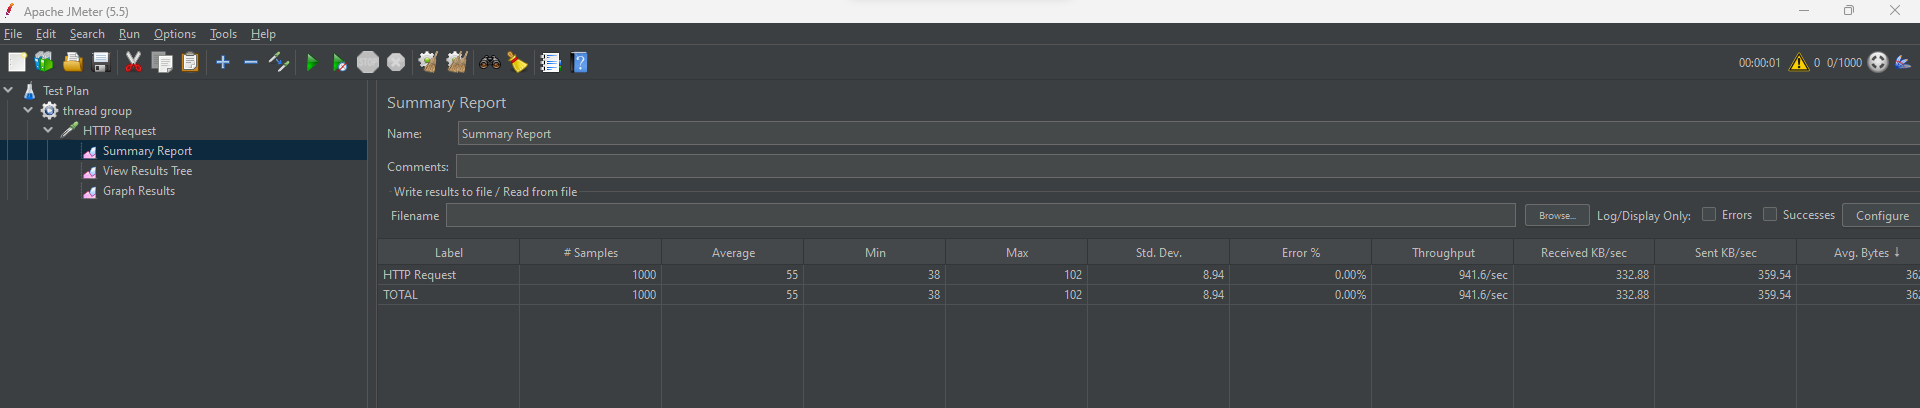
\includegraphics[scale=0.35]{1000_1.png}
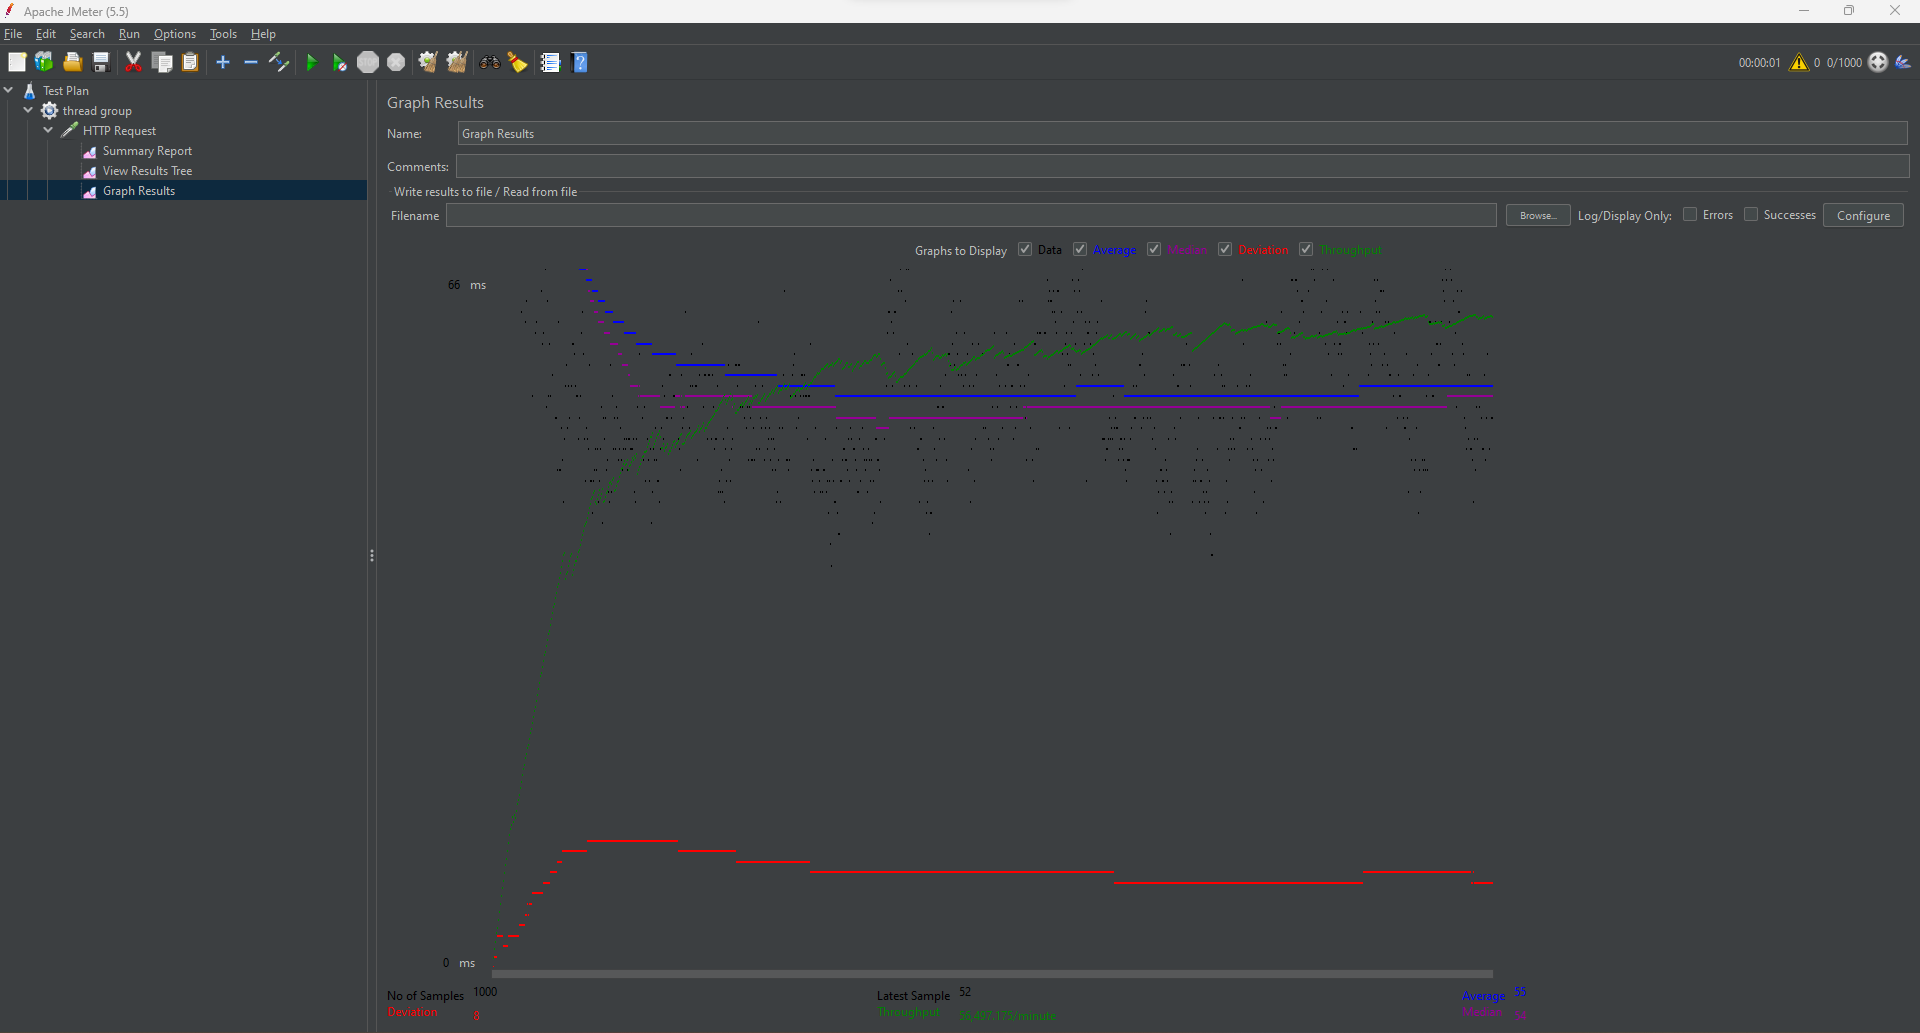
\includegraphics[scale=0.35]{1000_2.png}
\\
\newline
\\
設定執行序數量2000,系統反應平均為61ms,沒有錯誤 \\
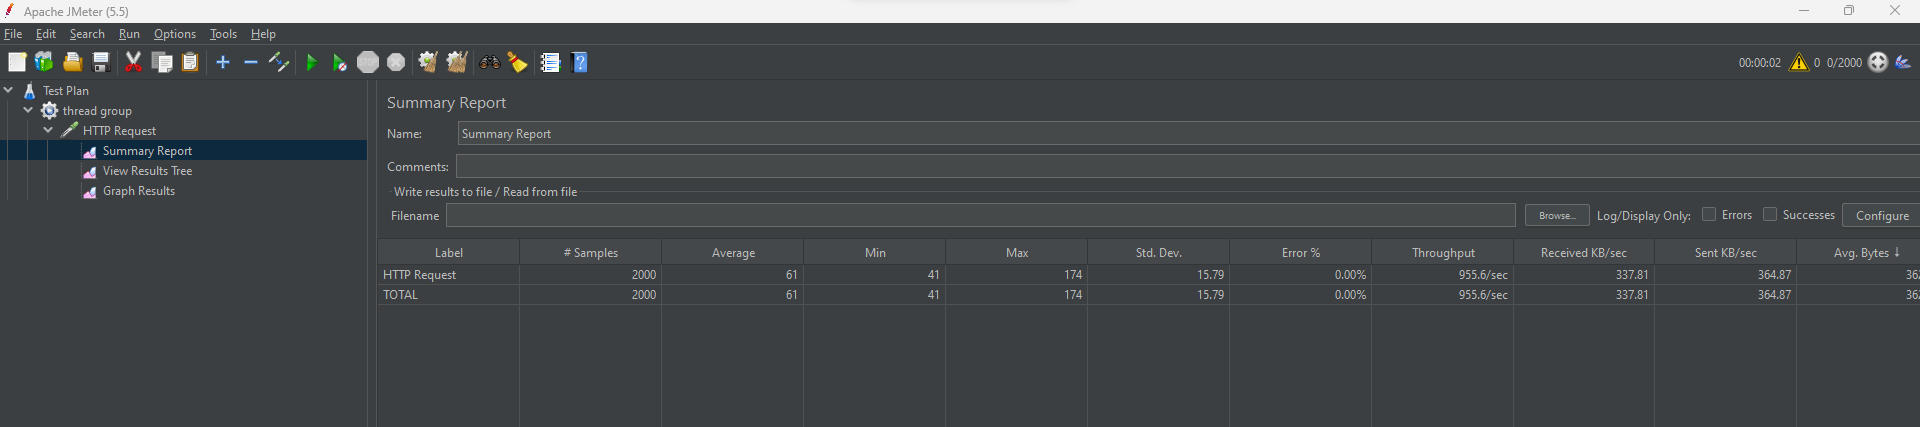
\includegraphics[scale=0.35]{2000_1.png}
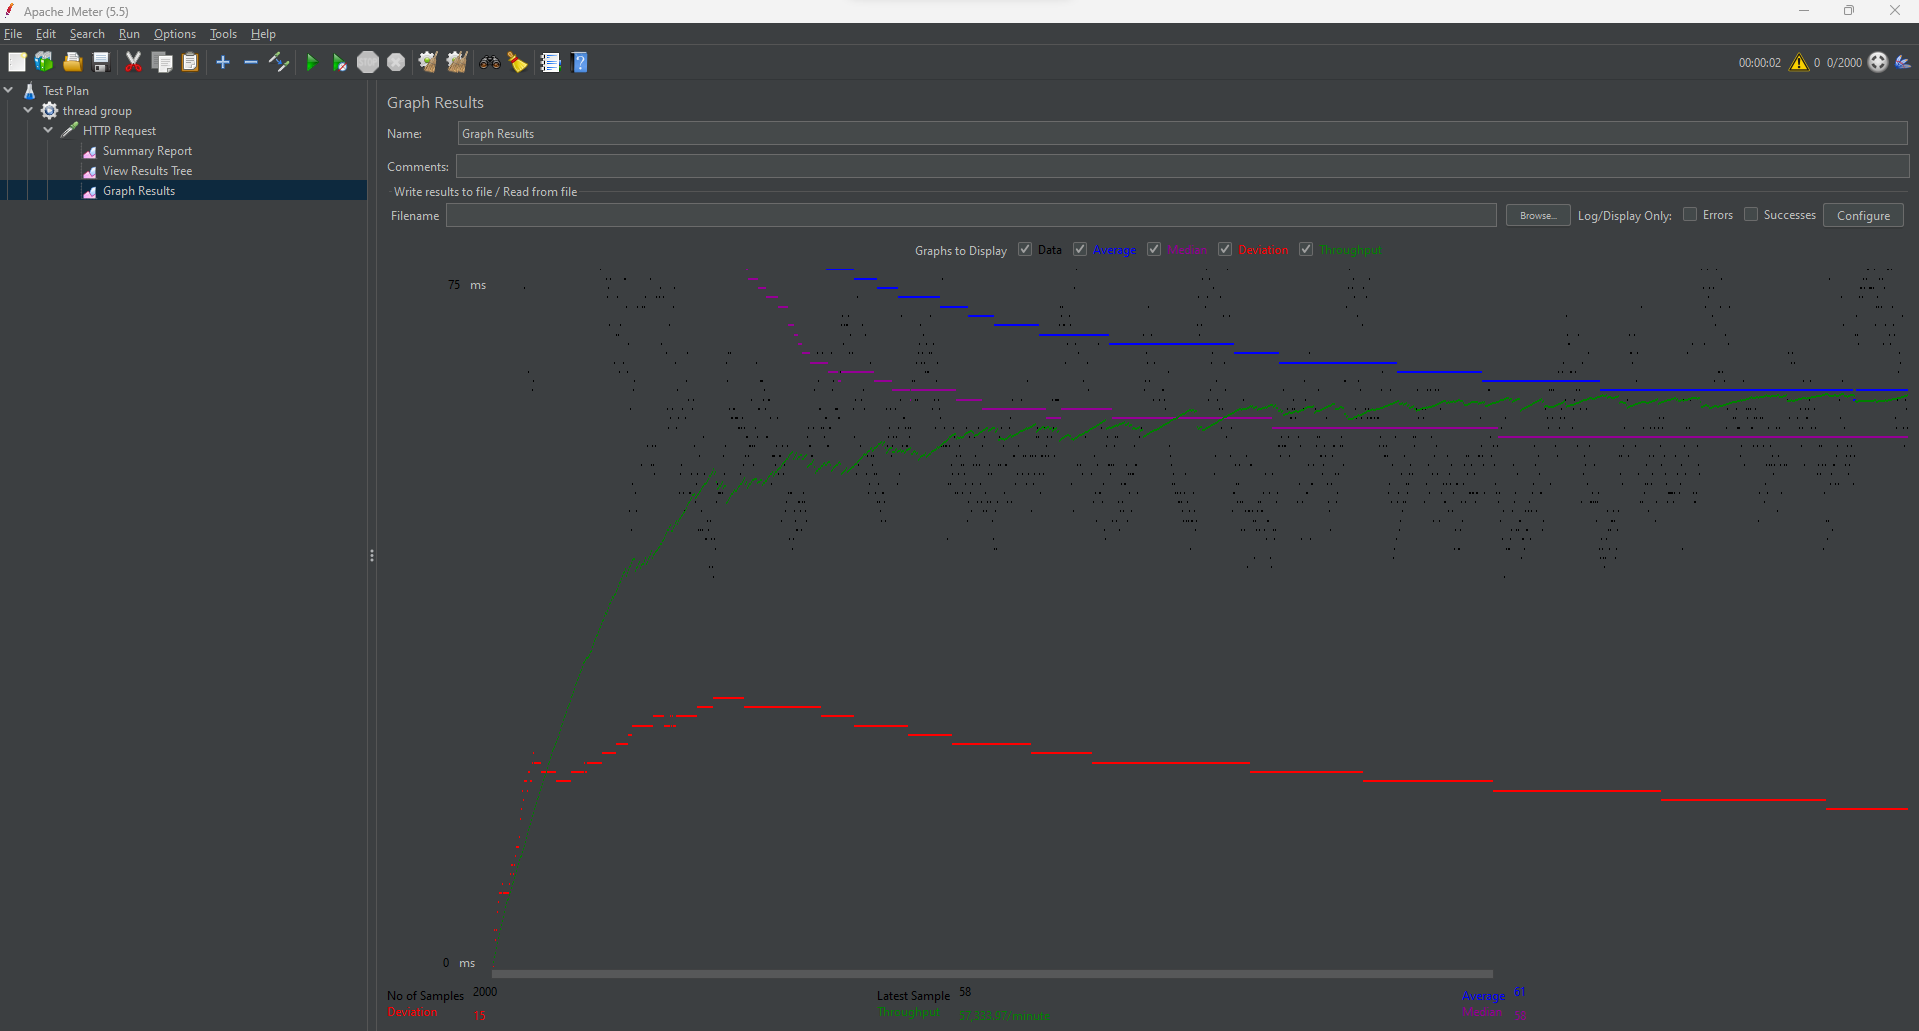
\includegraphics[scale=0.35]{2000_2.png}
\\
\newline
\\
設定執行序數量3000,出現錯誤 \\
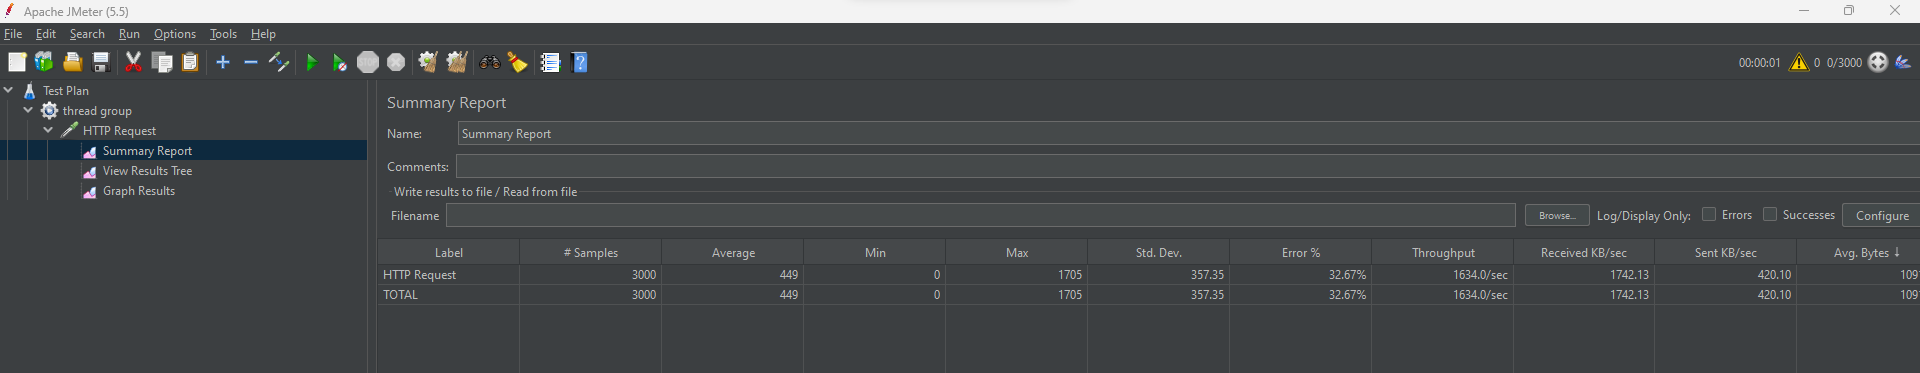
\includegraphics[scale=0.35]{3000.png}
\\
\newline
\\
\section*{6. 追溯表(Traceability Matrix)}
\begin{tabularx}{\textwidth}{ 
  |p{\dimexpr.4\linewidth-2\tabcolsep-1.33333\arrayrulewidth}%
  |p{\dimexpr.4\linewidth-2\tabcolsep-1.33333\arrayrulewidth}%
  |p{\dimexpr.2\linewidth-2\tabcolsep-1.33333\arrayrulewidth}|%
}
  \hline
  Req. No. & Test Case \#Verification & Verification \\
  \hline
  SCAF-FR-01 & SCAF-TC-01 & Verified \\
  \hline
  SCAF-FR-01 & SCAF-TC-02 & Verified \\
  \hline
  SCAF-FR-02 & SCAF-TC-03 & Verified \\
  \hline
  SCAF-FR-02 & SCAF-TC-04 & Verified \\
  \hline
  SCAF-FR-03 & SCAF-TC-05 & Verified \\
  \hline
  SCAF-FR-03 & SCAF-TC-06 & Verified \\
  \hline
  SCAF-FR-04 & SCAF-TC-07 & Verified \\
  \hline
  SCAF-FR-04 & SCAF-TC-08 & Verified \\
  \hline
  SCAF-FR-04 & SCAF-TC-09 & Verified \\
  \hline
  SCAF-FR-04 & SCAF-TC-10 & Verified \\
  \hline
  SCAF-FR-05 & SCAF-TC-11 & Verified \\
  \hline
  SCAF-FR-06 & SCAF-TC-12 & Verified \\
  \hline
  SCAF-FR-06 & SCAF-TC-13 & Verified \\
  \hline
  SCAF-FR-07 & SCAF-TC-14 & Verified \\
  \hline
  SCAF-FR-07 & SCAF-TC-15 & Verified \\
  \hline
  SCAF-FR-07 & SCAF-TC-16 & Verified \\
  \hline
  SCAF-FR-08 & SCAF-TC-17 & Verified \\
  \hline
  SCAF-FR-08 & SCAF-TC-18 & Verified \\
  \hline
  SCAF-FR-08 & SCAF-TC-19 & Verified \\
  \hline
  SCAF-FR-08 & SCAF-TC-20 & Verified \\
  \hline
  SCAF-FR-09 & SCAF-TC-21 & Verified \\
  \hline
  SCAF-FR-09 & SCAF-TC-22 & Verified \\
  \hline
  SCAF-FR-09 & SCAF-TC-23 & Verified \\
  \hline
  SCAF-FR-09 & SCAF-TC-24 & Verified \\
  \hline
  SCAF-FR-10 & SCAF-TC-25 & Verified \\
  \hline
  SCAF-FR-10 & SCAF-TC-26 & Verified \\
  \hline
  SCAF-FR-11 & SCAF-TC-27 & Verified \\
  \hline
  SCAF-FR-11 & SCAF-TC-28 & Verified \\
  \hline
  SCAF-FR-11 & SCAF-TC-29 & Verified \\
  \hline
  SCAF-FR-12 & SCAF-TC-30 & Verified \\
  \hline
  SCAF-FR-14 & SCAF-TC-31 & Verified \\
  \hline
  SCAF-FR-14 & SCAF-TC-32 & Verified \\
  \hline
  SCAF-FR-14 & SCAF-TC-33 & Verified \\
  \hline
  SCAF-FR-06 & SCAF-TC-34 & Verified \\
  \hline
  SCAF-FR-06 & SCAF-TC-35 & Verified \\
  \hline
\end{tabularx}
\newpage
\begin{tabularx}{\textwidth}{ 
  |p{\dimexpr.4\linewidth-2\tabcolsep-1.33333\arrayrulewidth}%
  |p{\dimexpr.4\linewidth-2\tabcolsep-1.33333\arrayrulewidth}%
  |p{\dimexpr.2\linewidth-2\tabcolsep-1.33333\arrayrulewidth}|%
}
  \hline
  SCAF-FR-01 & SCAF-TC-36 & Verified \\
  \hline
  SCAF-FR-02 & SCAF-TC-37 & Verified \\
  \hline
  SCAF-FR-03 & SCAF-TC-38 & Verified \\
  \hline
  SCAF-FR-06 & SCAF-TC-39 & Verified \\
  \hline
  SCAF-FR-07 & SCAF-TC-40 & Verified \\
  \hline
\end{tabularx}
\end{document}




